\subsection{L'ogica de juego}

1- Manejo de las Cartas
=======================

Escala:
0 01E
1 01B
2 07E
3 07O
4 03O,03C,03B,03E
5 02O,02C,02B,02E
6 01O,01C
7 12O,12C,12B,12E
8 11O,11C,11B,11E
9 10O,10c,10B,10E
10  07B,07C
11  06O,06C,06B,06E
12  05O,05C,05B,05E
13  04O,04C,04B,04E

  Se define un orden parcial entre las cartas, que indica el valor relativo entre ellas. Esto nos va a servir para despues comparar, en base a las cartas en la mesa, qui'en "mat'o", y a qui'en le corresponde jugar.

  * Para ver qui'en gana la mano, buscamos las dos cartas que est'an sobre la mesa y vemos cu'al tiene el nivel m'as alto (esa es la que gana la mano). En caso de estar en niveles iguales hay parda y le toca jugar al jugador que es mano.
carta (la mano).


2- Manejo de Cantos
===================

Envido
------
  * Se puede cantar Envido hasta antes de jugar la primera mano
  * Se puede seguir contestando hasta que se diga "Quiero"; ac'a se procede a ver qu'e cartas son del mismo palo y se suman los valores (en caso de tenes flor se suman los dos m'as altos), o "No Quiero"; no cuento nada y sigue el juego.
  * Si se cant'o "Truco" no se puede cantar "Envido"
  * Si ya se dijo "Quiero" o "No Quiero", no se puede seguir cantando.

Truco
-----
  * Se puede cantar en cualquier mano e inclusive antes de jugar la primera carta.
  * El ganador de 2 de 3 manos es el que gana la mano.
  * Una vez que los 2 jugaron las 3 cartas no se puede cantar "Truco".

\begin{figure}
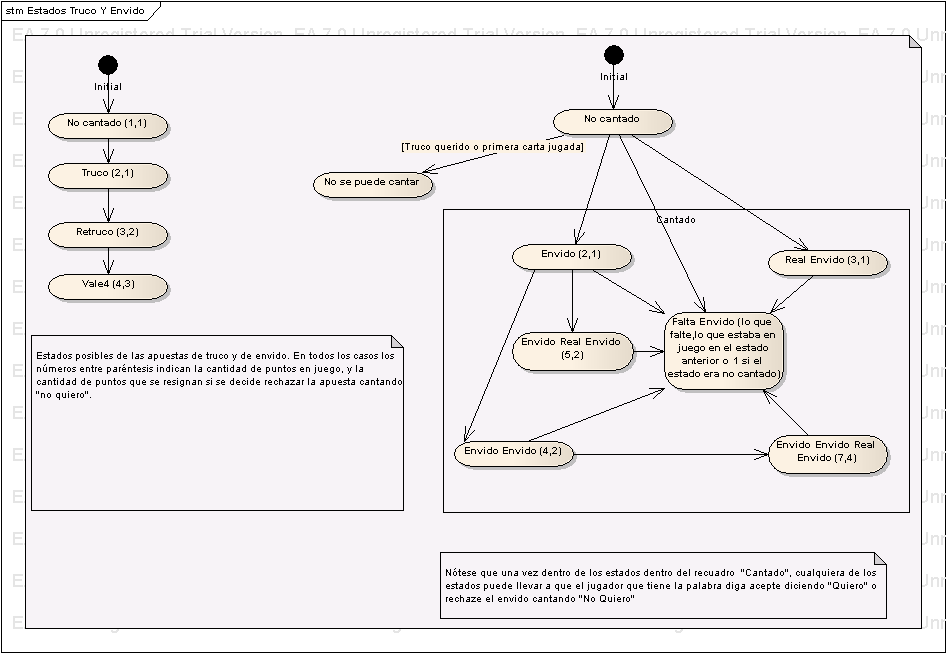
\includegraphics{Estados Truco Y Envido.png}
\end{figure}
\begin{figure}
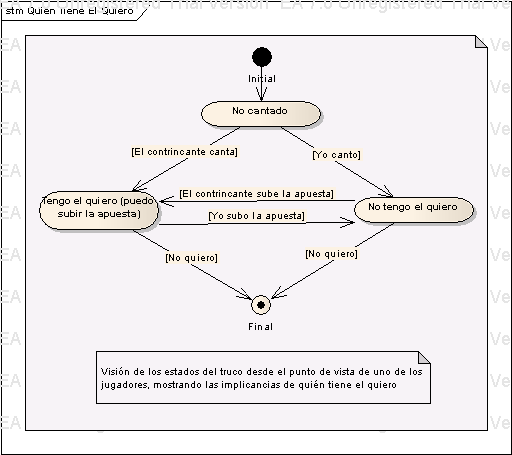
\includegraphics{Quien Tiene El Quiero.png}
\end{figure}

* Los cantos deben manejarse como interrupciones. Un jugador puede cantar "Truco" habiendo jugado su carta o no. No es asi el caso del "Envido"; aca hay que controlar que el jugador tenga el token (le toque jugar) y no haya tirado su carta.


3- Registros a Tener en Cuenta:
==============================

  * Cantidad de Manos Ganadas
  * Si se cant'o "Envido"
  * Si se cant'o "Truco"
  * Al finalizar la mano:
    - Si se cant'o "Envido" me fijo si en las cartas sobre la mesa est'an los puntos del "Envido". Si no, muestro las que faltan aunque se haya ido al mazo.
    - Si se fue al mazo (o se canta "Truco" y no se quiere), entonces no se deben mostrar las cartas que no se hayan jugado a menos que ocurra el caso anterior.


4- Decisiones de Implementaci'on:
===============================

** Se van a necesitar las siguientes variables para saber en que estado estamos dentro de Envido durante la
partida:

** Envido:
   ------
  Una variable EstadoEnvido que va a asumir los valores:
    0, si no se canto nada
    1, si se canto Envido
    2, si se canto Envido Envido
    3, si se canto Real Envido
    4, si se canto Falta Envido
    5, si ya no se puede seguir cantando (si el jugador respondio "Quiero" o " No Quiero")
  Una variable que almacene la cantidad de puntos en juego si se dice Quiero (PtosQuieroEnv)
  Una variable que almacene la cantidad de puntos en juego si se dice No Quiero (PtosNQuieroEnv)
  Una variable que me indique si puedo redoblar la apuesta del Envido (Es decir, si tengo el Quiero, PuedoCantarEnv)

Nota:
  La cantidad de Puntos en juego si se dice "No Quiero" es la cantidad de cantos que se hayan efectuado y la cantidad
de puntos en juego si se dice "Quiero" es sumar 2 si se canta Envido, 3 si se canta Real Envido. Se tomo esta decision ya quela cantidad de puntos en juego si se canta Envido, Envido, Real Envido no es la misma que si se canta Envido, Real Envido.

  Supongamos que la variable PtosQuieroEnv no existe y que manejamos el Envido con las otras dos variables. En el primer caso, la variable PtosNQuieroEnv tendria un valor 3 y en el segundo caso 2. La variable EstadoEnvido en el primer caso, pasaria del estado 0 al 1, luego al 2 y finalmente el 3; y en el segundo, pasaria del estado 0 al 1 y finalmente al 3. Ahora, cuando computemos los puntos en juego, suponiendo que se dijo "Quiero" a partir de EstadoEnv, en los dos casos terminaria con el mismo valor!, lo cual es incorrecto. Es por esto que se opto por tener un registro de las estapas del Envido en la que se encuentra (EstadoEnv), la cantidad de puntos en juego si se sice "Quiero" (esto soluciona el problema antes mencionado), y la cantidad de puntos en juego si se dice "No Quiero" que sirve para contar la cantidad de cantos que se efectuaron.

** Truco:
   -----
  Una variable EstadoTruco que va a asumir los siguientes valores:
    0, si no se canto nada
    1, si se canto Truco
    2, si se canto Re Truco
    3, si se canto Vale Cuatro
    4, si ya no se puede seguir cantando (si el jugador respondio "Quiero" o "No Quiero")
  Una variable que cuente los puntos del truco en caso que la respuesta sea "Quiero" (PtosQuieroTru)
  Una variable que cuente los puntos del truco en caso que la respuesta sea "No Quiero" (PtosNQuieroTru)
  Una variable que me indique si puedo redoblar la apuesta del Truco (Es decir, si tengo el Quiero, PuedoCantarTru)

Nota:
  Tanto los puntos del truco querido como los del no querido se van incrementando de a uno. La diferencia esta en que PtosQuieroTru de 0 pasa al valor 2; en cambio, PtosNQuieroTru pasa de 0 a 1.
